% IEEE Journal Paper Template
\documentclass[journal]{IEEEtran}

% Packages
\usepackage{amsmath,amssymb,amsfonts}
\usepackage{algorithmic}
\usepackage{algorithm}
\usepackage{graphicx}
\usepackage[nocompress]{cite}
\usepackage{url}
\usepackage{multirow}
\usepackage{amsthm}
\usepackage{placeins}
\newtheorem{theorem}{Theorem}
\newtheorem{proposition}{Proposition}
\newtheorem{assumption}{Assumption}

\newcommand{\PaperTitle}{Shapley-Guided Energy-Constrained Client Scheduling for Federated Learning under Non-IID Data}
\pdfinfo{
  /Title (\PaperTitle)
}

\begin{document}

\title{\PaperTitle}

\author{}

\maketitle

\begin{abstract}
Client selection in federated learning (FL) needs to consider both learning value and resource sustainability. In non-IID data settings, some clients can provide more useful updates, but selecting these clients too frequently may bring long-term energy imbalance in wireless edge systems. This paper proposes a Shapley-guided energy-constrained scheduler for synchronous cross-device FL. The server keeps persistent Shapley contribution estimates by a lightweight complementary-contribution sampler, records per-client energy pressure by virtual queues, and selects feasible clients according to a score-based distribution. We also add an auxiliary channel-noise diagnostic module, which clips client updates and models receiver-side channel uncertainty as equivalent Gaussian perturbation on the released aggregate. This module gives a common noisy-release reference for noise--utility analysis. We characterize the selection effect caused by the proposed score rule. On CIFAR-10 with $\alpha=0.1$, three seeds, and $T=100$ rounds, the proposed scheduler obtains the best last-5-round accuracy among the compared baselines while keeping explicit energy accounting. Ablation results show that the Shapley signal improves the deployable energy-aware scheduler, and the virtual queue provides the long-term energy-accounting mechanism. Sensitivity studies further examine data heterogeneity, sampling budget, and channel-noise diagnostics.
\end{abstract}

\begin{IEEEkeywords}
Federated learning, client selection, Shapley value, energy-constrained scheduling, non-IID data, virtual queue, channel noise accounting
\end{IEEEkeywords}

\section{Introduction}

Federated learning (FL) \cite{mcmahan2017communication} allows distributed clients to train a shared model without sending raw data to a central server. It has become an important framework for privacy-aware distributed learning \cite{kairouz2021advances}. This framework is suitable for mobile-edge and Internet-of-Things systems, because data are generated on devices and direct data collection may be costly or privacy-sensitive \cite{lim2020federated,khan2021federated}. Wireless-network studies also show that communication constraints and channel variation are closely related to the learning process in edge FL \cite{chen2021distributed}. In a typical cross-device FL system, the server repeatedly selects a subset of clients, broadcasts the current global model, receives local updates, and aggregates them into the next global model. Therefore, client selection is not only an implementation detail. It directly determines which data, channels, and devices participate in the learning trajectory.

In practical wireless FL, client participation is more than a random sampling operation. Edge clients are different in data distribution, channel condition, residual battery state, and expected energy consumption. Early mobile-edge FL work showed that heterogeneous resources make client selection an important design factor \cite{nishio2019client}. Later resource-constrained and wireless FL studies connected participation, communication allocation, and scheduling policy with training efficiency \cite{wang2019adaptive,chen2021joint,yang2020scheduling}. A client with informative non-IID data may improve the model, but selecting this client repeatedly under poor wireless links may consume too much energy and reduce long-term participation sustainability. On the other hand, a client with a good channel may be cheap to schedule but may not be useful enough for the current learning task.

This paper studies synchronous cross-device FL with one parameter server, image-classification tasks, and wireless edge clients. The per-round energy consumption contains a Rayleigh-fading transmission term and a CPU-based local-computation term. The main objective is to make contribution-aware scheduling under long-term energy pressure. We also report a lightweight channel-noise diagnostic for the released aggregate. The uploaded updates are clipped to bound the perturbation scale, and receiver-side channel uncertainty is modeled as equivalent Gaussian perturbation. This diagnostic provides the same noisy wireless-release condition for different schedulers and helps interpret the noise--utility effect of channel perturbation. The study focuses on synchronous scheduling, energy accounting, and channel-aware noisy-release evaluation.

The client selection problem becomes more difficult under non-independent and non-identically distributed (non-IID) data. Data heterogeneity makes local updates have different contributions to the global model and may slow down FedAvg convergence \cite{li2020convergence}. Recent surveys also point out that non-IID data are still a common obstacle for practical FL deployment \cite{lu2024noniidsurvey}. Uniform random participation, as used in FedAvg, ignores this statistical difference. Existing client selection methods improve random sampling by using statistical utility and system efficiency \cite{lai2021oort}, non-IID-aware mobile-edge selection criteria \cite{zhang2021client}, or group structure under industrial IoT heterogeneity \cite{li2022fedgs}. These signals are useful, but they are still indirect measurements of a client's marginal contribution to the aggregated model.

At the same time, contribution-aware scheduling alone is not enough for wireless edge systems. Clients communicate through time-varying channels and have limited energy budgets. If a scheduler always prefers high-contribution clients, it may repeatedly consume the same devices. Long-term wireless FL studies show that temporal selection and bandwidth allocation affect both communication cost and learning result \cite{xu2021client}. Energy-constrained client selection has also been studied by long-horizon bandit and AIoT-oriented formulations \cite{zhu2024cmabenergy,zhang2025eecsfl}. Therefore, an online scheduling mechanism is needed to jointly consider statistical contribution, current channel opportunity, residual battery state, and long-term energy pressure.

Motivated by this gap, this paper develops a \textbf{Shapley-guided channel- and energy-aware client scheduler}. The server estimates client contribution through a complementary-contribution-inspired Shapley sampler on a validation proxy, maintains persistent contribution statistics across rounds, filters clients by residual energy, and samples feasible clients according to a score-based utility-minus-queue distribution. The utility term combines contribution, residual battery state, and channel quality, while drift-inspired virtual queues record cumulative energy-budget pressure and penalize clients whose historical energy consumption is persistently high.

The proposed mechanism has two core components and one auxiliary diagnostic component. First, the complementary-contribution Shapley estimator provides a contribution-oriented signal. Compared with local loss alone, this signal is more directly related to model utility, and it can reuse coalition utilities across clients. Second, the channel- and energy-aware score helps the server balance good wireless opportunities and long-term participation pressure. The auxiliary channel-noise diagnostic reports how equivalent receiver-side perturbation changes the noise--utility reference value under a shared noisy-release setting. We characterize the selection effect induced by the proposed score rule and give a finite-time energy-accounting property for the implemented virtual queues.

The main contributions of this paper are summarized as follows:

\begin{enumerate}
\item We develop a persistent Shapley-based contribution estimator for non-IID FL, implemented with a complementary-contribution sampling routine, and integrate it into online client scheduling.

\item We design a score-based scheduling rule that jointly balances contribution, residual battery state, channel quality, and long-term virtual-queue pressure.

\item We characterize the score-based selection process, discuss the estimator's sampling behavior, and provide a finite-time energy-accounting property for the virtual queue recursion.

\item We validate the proposed scheduler on CIFAR-10 through ablation, heterogeneity sensitivity, sampling-budget sensitivity, and channel-noise diagnostic analysis, showing gains over representative baselines under the tested non-IID setting.
\end{enumerate}

\begin{figure*}[!t]
    \centering
    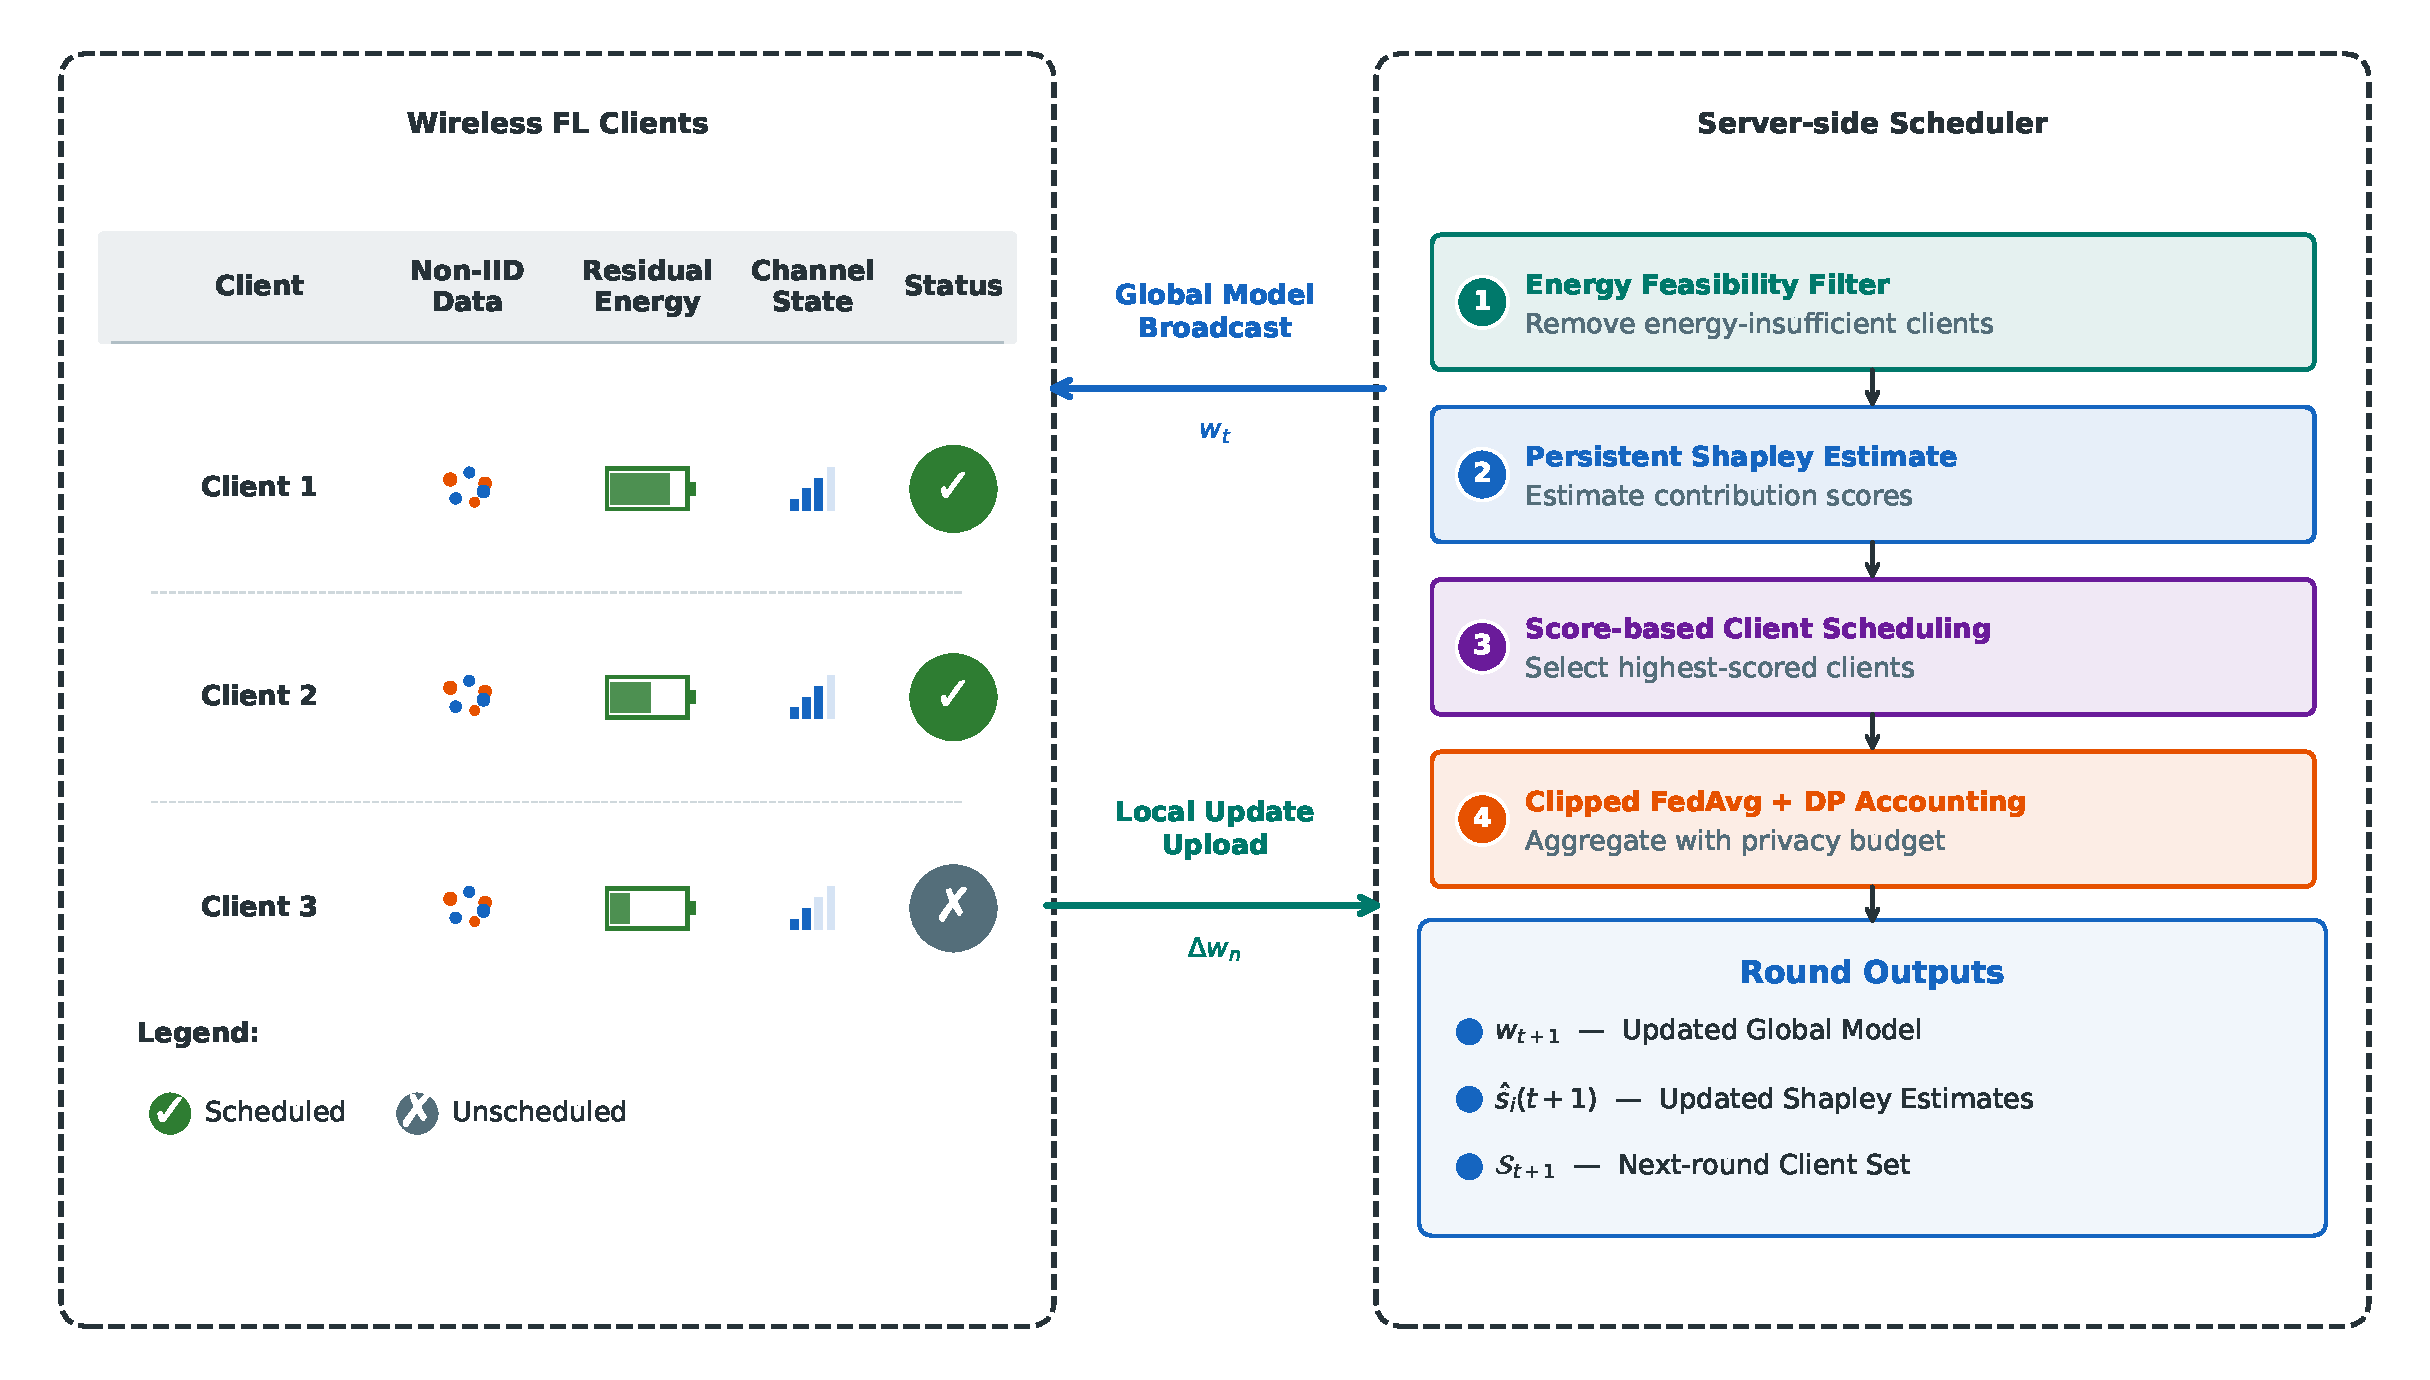
\includegraphics[width=0.95\textwidth]{figures/framework_overview.pdf}
    \caption{Conceptual framework of the proposed Shapley-guided energy-constrained client scheduling mechanism for wireless federated learning under non-IID data. The server combines persistent Shapley estimates, residual energy, channel state, and virtual-queue pressure to select clients, aggregate clipped updates, and refresh the scheduling state for the next round.}
    \label{fig:framework_overview}
\end{figure*}

The remainder of this paper is organized as follows. Section~II reviews related work. Section~\ref{sec:system} presents the FL system model, wireless energy model, and scheduling problem. Section~\ref{sec:method} develops the Shapley-guided energy-aware scheduling mechanism, including queue-based scoring, contribution estimation, client selection, aggregation, and state refresh. Section~\ref{sec:analysis} characterizes the score-based selection mechanism and the energy-accounting property. Section~\ref{sec:experiments} presents simulation results. Section~\ref{sec:conclusion} concludes the paper.

\section{Related Work}
\label{sec:related}

\subsection{Federated Learning and Client Selection}

FedAvg established the standard FL protocol. In this protocol, a server samples clients, broadcasts the current global model, and averages the returned local models. Because of its simplicity, FedAvg is widely used as a baseline. However, random participation can be inefficient when clients have different data distributions, computation capabilities, and communication conditions. FedProx \cite{li2020federated} addresses statistical heterogeneity by adding a proximal regularizer to local training. Therefore, it is still a useful heterogeneity-aware baseline even when the main research question is client scheduling. These limitations motivate client-selection methods that use heterogeneity to select more useful or more efficient clients.

Representative selection schemes use different proxies to describe client quality. Oort combines statistical utility, system efficiency, and exploration. Mobile-edge and industrial-IoT studies select clients according to resource feasibility, data heterogeneity, or group structure. Fairness-aware and efficiency-oriented selection schemes show that client choice can influence convergence behavior and participation balance \cite{huang2021efficiency}. Quality-aware and multicriteria selection also indicate that client scheduling is usually a multi-objective decision, not only an accuracy heuristic \cite{deng2022auction,abdulrahman2021fedmccs}. These methods show that client selection can affect convergence and final accuracy. However, their signals are usually short-horizon proxies, such as loss, latency, data distribution, or heuristic utility. Different from them, our scheduler uses a contribution-oriented signal and combines it with long-term energy accounting. Thus, the selection rule reflects both round-level learning value and accumulated device burden.

\subsection{Contribution-Based Client Selection}

Shapley values provide a game-theoretic measure for the average marginal contribution of each participant. They have been widely used in data valuation, incentive design, and fairness analysis in collaborative learning. In FL, Shapley-style valuation can identify clients whose updates are more useful for the global model, especially under non-IID data where update quality is quite different across clients. Recent work has further improved FL client sampling with modified Shapley mechanisms \cite{wu2026fedmsv}.

The main obstacle is computational cost. Exact Shapley evaluation needs to enumerate all coalitions, so it is impractical for cross-device FL. Recent approximation work has shown that complementary-contribution stratified sampling can reuse one coalition evaluation across multiple players and reduce repeated utility computation \cite{sun2024complementary}. Following this idea, we use a lightweight complementary-contribution sampler and maintain persistent cross-round averages. In this way, the contribution estimate can be used as an online scheduling signal. This is different from purely post-training valuation, because the estimated contribution is fed back into the next-round client selection process.

\subsection{Resource-Aware Federated Learning}

Wireless FL needs to consider channel variation, energy consumption, bandwidth limitation, and device availability. One line of work studies over-the-air aggregation, where waveform superposition is used to reduce aggregation latency in wireless learning systems \cite{yang2020otafl,amiri2020machine}. Later OTA-FL studies further examine broadband analog aggregation and update-aware device scheduling. These studies show that fading, receive noise, and power control can directly influence convergence behavior \cite{zhu2020broadband,amiri2021updateaware}.

Beyond aggregation design, wireless scheduling studies use channel state or gradient importance to decide which devices should transmit in each round \cite{ren2020scheduling,du2023gradient}. Data-importance and data-aware schedulers further show that communication efficiency depends not only on channel quality, but also on the learning value of selected clients \cite{su2022datachannel}. Related data-aware device scheduling studies obtain a similar conclusion from the perspective of edge learning and communication-efficient user participation \cite{liu2021data,taik2022data}. Together with the long-term and multicriteria studies above, these works show that learning performance and communication efficiency should be optimized together.

Our work follows this joint-design perspective and uses a long-horizon control structure. The scheduler maintains per-client virtual queues to accumulate energy-budget pressure over rounds. It also uses instantaneous battery state, channel feasibility, and learning utility. The queue mechanism converts repeated energy overuse into a future selection penalty. Therefore, the scheduler can allow occasional expensive selections but discourage persistent depletion of the same clients.

\subsection{Channel Noise in Wireless Federated Learning}

Wireless FL is different from purely wired or server-side simulations, because the aggregate observed at the receiver can be affected by propagation noise, fading, and receiver uncertainty. In over-the-air FL, this effect is a part of the aggregation mechanism itself. Prior studies have shown that receive noise and power control can change the learning dynamics of wireless aggregation systems \cite{yang2020otafl,amiri2020machine,zhu2020broadband,amiri2021updateaware}. Related work also connects physical-layer channel noise with privacy-aware aggregation when the wireless transmission model and privacy budget are jointly specified \cite{yan2023otafedavgprivacy}.

In this paper, channel noise is used as a diagnostic component for digital FL scheduling experiments. The module represents receiver-side propagation uncertainty as an equivalent perturbation on the clipped aggregate. Therefore, all schedulers are evaluated under the same noisy wireless-release setting. This gives the experiments a common wireless-release reference: the compared methods are different in client scheduling, while the receiver-side perturbation condition is fixed.

Table~\ref{tab:related} compares the main design features of representative selection schemes. The GCA row denotes the gradient/channel-aware scheduling family that motivates our digital-FL GCA-inspired comparator. The auxiliary channel-noise diagnostic is applied uniformly in the experiments, so it is not counted as a feature of the baseline schedulers.

\begin{table}[t]
\centering
\caption{Feature comparison of client-selection schemes.}
\label{tab:related}
\scriptsize
\setlength{\tabcolsep}{2pt}
\begin{tabular}{l|c|c|c|c}
\hline
\textbf{Method} & \textbf{Selection Signal} & \textbf{Energy} & \textbf{Learning} & \textbf{Long-Term} \\
 & & \textbf{Aware} & \textbf{Signal} & \textbf{Queue} \\
\hline
FedAvg & uniform random & $\times$ & $\times$ & $\times$ \\
FedProx & random + prox term & $\times$ & $\times$ & $\times$ \\
Oort & utility + system & one-shot & utility proxy & $\times$ \\
GCA-inspired & grad./loss + channel + energy & one-shot & grad. proxy & $\times$ \\
\textbf{Ours} & Shapley sampler + queue & long-term & Shapley & $\checkmark$ \\
\hline
\end{tabular}
\end{table}

\section{System Model and Problem Formulation}
\label{sec:system}

\begin{table}[t]
\centering
\caption{List of Main Notations}
\label{tab:notation}
\small
\setlength{\tabcolsep}{3pt}
\begin{tabular}{c p{0.68\columnwidth}}
\hline
\textbf{Notation} & \textbf{Definition} \\
\hline
$N$ & Total number of clients \\
$K$ & Per-round client selection budget \\
$T$ & Total number of communication rounds \\
$\mathcal{S}_t$ & Subset of selected clients in round $t$ \\
$a_n(t)$ & Binary selection indicator of client $n$ in round $t$ \\
$\varphi_n(t)$ & Persistent Shapley estimate available for client $n$ at the start of round $t$ \\
$U_n(t)$ & Instantaneous scheduling utility of client $n$ \\
$\mathrm{Score}_n(t)$ & Utility-minus-queue score used for scheduling \\
$E_n(t)$ & Energy consumption of client $n$ in round $t$ \\
$E_{\text{remain},n}(t)$ & Residual battery energy of client $n$ at the start of round $t$ \\
$\bar{E}$ & Per-round average energy budget for each client \\
$B_n(t)$ & Normalized residual-battery state used in the scheduling utility \\
$h_n(t)$ & Complex wireless channel coefficient of client $n$ in round $t$ \\
$\chi_n(t)$ & Normalized channel-quality signal \\
$W$ & Uplink bandwidth allocated to one selected client \\
$L_{\mathrm{up}}$ & Uplink payload size of one model update \\
$\tau_{\mathrm{up}}$ & Uplink transmission-duration budget \\
$N_0$ & Receiver noise power spectral density \\
$P_{\mathrm{cir}}$ & Circuit power consumed during uplink transmission \\
$P_{\max}$ & Peak transmit-power cap used under rare deep fades \\
$Q_n(t)$ & Virtual energy-pressure queue of client $n$ \\
$V$ & Scheduler control parameter \\
$\lambda_s,\lambda_b,\lambda_c$ & Utility weights for Shapley contribution, residual battery, and channel quality \\
$\alpha$ & Dirichlet concentration parameter controlling non-IID skew \\
$C_t$ & Update clipping norm used to bound sensitivity in round $t$ \\
\hline
\end{tabular}
\end{table}

\subsection{Federated Learning Framework}

We consider a synchronous FL system with one parameter server and $N$ wireless edge clients, denoted by $\mathcal{N}=\{1,2,\ldots,N\}$. Client $n$ stores a private dataset $\mathcal{D}_n$ with $|\mathcal{D}_n|$ samples. It participates in training only by sending model updates. The learning objective is the standard data-size-weighted average of local empirical risks:
\begin{equation}
F(w)=\sum_{n=1}^{N}p_nF_n(w),
\end{equation}
where $p_n=|\mathcal{D}_n|/\sum_{i=1}^{N}|\mathcal{D}_i|$ denotes the data fraction of client $n$. The local objective is
\begin{equation}
F_n(w)=\mathbb{E}_{(x,y)\sim\mathcal{D}_n}[\ell(w;x,y)].
\end{equation}
Here $w$ is the model parameter and $\ell(w;x,y)$ is the sample-wise training loss.

Training proceeds over $T$ communication rounds. At the beginning of round $t$, the server selects a subset $\mathcal{S}_t\subseteq\mathcal{N}$ with $|\mathcal{S}_t|=K_t\leq K\ll N$. Then the server broadcasts the current model $w_t$ to the selected clients. Each selected client runs $\tau$ local SGD epochs, and client $n$ returns a local model $\tilde{w}_n^{t+1}$. The server aggregates the returned models by weighted FedAvg:
\begin{equation}
w_{t+1}=\sum_{n\in\mathcal{S}_t}
\frac{|\mathcal{D}_n|}{\sum_{i\in\mathcal{S}_t}|\mathcal{D}_i|}
\tilde{w}_n^{t+1}.
\end{equation}
This paper focuses on how to construct $\mathcal{S}_t$ when statistical utility, wireless channel opportunity, residual battery state, and long-term energy sustainability are coupled together.

For post-round contribution evaluation, the server holds a small validation proxy $\mathcal{D}_{\text{val}}$, which is disjoint from local training partitions and the test set. This proxy is fixed before training and does not require additional client upload during FL. In deployment, it can be replaced by a public reference set or a privacy-preserving validation protocol. The simulation setting is described in Section~\ref{sec:experiments}.

\subsection{Data Heterogeneity and Wireless Energy Model}

We model statistical heterogeneity by the standard Dirichlet partition used in FL experiments. For a classification task with $C$ classes, each client receives a class-proportion vector drawn from $\mathrm{Dir}(\alpha)$. A smaller $\alpha$ creates stronger non-IID skew, and a larger $\alpha$ is closer to the i.i.d. case.

Each client communicates with the server over a time-varying Rayleigh fading uplink with coefficient $h_n(t)$ and power gain $|h_n(t)|^2$. The total round energy consumption contains an uplink transmission component and a local-computation component. To connect the scheduling cost to a physical wireless link, suppose that one selected client uploads a model-update payload of $L_{\mathrm{up}}$ bits within a transmission-duration budget $\tau_{\mathrm{up}}$ over bandwidth $W$. Under Shannon-rate inversion, the minimum transmit power needed to support rate $L_{\mathrm{up}}/\tau_{\mathrm{up}}$ is
\begin{equation}
P_{\mathrm{tx},n}(t)
=
\frac{N_0 W}{|h_n(t)|^2}
\left(2^{\frac{L_{\mathrm{up}}}{W\tau_{\mathrm{up}}}}-1\right),
\end{equation}
where $N_0$ is the receiver noise power spectral density. The corresponding uplink energy, including a circuit-power term and a peak-power/rare-fade cap, is
\begin{equation}
E_{\text{trans},n}(t)
=
\tau_{\mathrm{up}}\left(
\min\{P_{\mathrm{tx},n}(t),P_{\max}\}
+P_{\mathrm{cir}}
\right).
\end{equation}
This expression shows that poor channel realizations increase the energy required for reliable upload. In the simulator, constants shared by all clients are absorbed into a normalized channel-dependent cost. Therefore, the implemented transmission term is equivalent to a capped inverse-channel proxy after normalization. The local computation component is
\begin{equation}
E_{\text{comp},n}(t)=\tau\cdot\kappa\cdot f^2\cdot C_{\text{cyc}}\cdot D_n.
\end{equation}
The per-round energy consumption is then
\begin{equation}
E_n(t)=E_{\text{trans},n}(t)+E_{\text{comp},n}(t).
\end{equation}
Here $P_{\max}$ clips rare extreme transmission costs under deep fading, $\kappa$ is the effective switched capacitance coefficient, $f$ is the CPU frequency, $C_{\text{cyc}}$ is the number of cycles per sample, and $D_n=|\mathcal{D}_n|$. The scheduling algorithm only needs a predicted per-round energy cost $E_n(t)$. Therefore, richer link-budget terms, such as path loss, client-specific bandwidth allocation, or retransmission overhead, can be incorporated by replacing $E_{\text{trans},n}(t)$ without changing the queue-based scheduler.

Each client maintains a residual energy state initialized at $E_{\text{init}}$. Selected clients spend $E_n(t)$ in round $t$. Clients whose residual energy falls below $E_{\text{threshold}}$ are excluded from future candidate sets. This feasibility threshold handles immediate battery exhaustion. The virtual queue introduced later captures long-term energy-budget pressure.

The residual battery state evolves as
\begin{equation}
E_{\text{remain},n}(t+1)=E_{\text{remain},n}(t)-a_n(t)E_n(t).
\end{equation}
If client $n$ is not selected in round $t$, then $a_n(t)=0$ and its residual energy remains unchanged.

\subsection{Problem Formulation}
\label{sec:problem}

The central scheduling question is how to select clients when learning contribution, channel quality, residual battery state, and long-term energy sustainability are coupled. We write the resource-aware scheduling objective as:
\begin{subequations}
\begin{align}
\max_{\{a_n(t)\}}\quad
&\sum_{t=1}^{T}\sum_{n=1}^{N}a_n(t)U_n(t)\\
\text{s.t.}\quad
&\sum_{n=1}^{N}a_n(t)\leq K,\quad \forall t,\\
&\frac{1}{T}\sum_{t=1}^{T}a_n(t)E_n(t)\leq \bar{E},\quad \forall n,\\
&a_n(t)\in\{0,1\},\quad \forall n,t.
\end{align}
\end{subequations}
Here $U_n(t)$ denotes the instantaneous utility induced by contribution, residual battery state, and channel quality. $\bar{E}$ is the per-round average energy budget. The contribution component cannot be known in advance. In the online scheduler, it is instantiated by the persistent Shapley estimate accumulated from previous selected rounds.

\section{Shapley-Guided Energy-Aware Scheduling Mechanism}
\label{sec:method}

This section develops the proposed online scheduler based on the problem in Section~\ref{sec:system}. The mechanism has four connected components. First, a virtual queue converts the long-term energy constraint into a round-start scheduling penalty. Second, a persistent Shapley estimate provides a contribution signal before selection. Third, the server combines contribution, residual battery, channel quality, and queue pressure into a score-based selection distribution. Finally, after local training, the server aggregates clipped updates, applies the shared channel-noise diagnostic, and refreshes the contribution and energy states for the next round.

\subsection{Queue-Based Energy-Aware Score}

The resource-aware problem couples decisions across rounds through the average-energy constraints. It cannot be solved directly without knowing future channel states, energy evolution, and contribution estimates. Therefore, we introduce a virtual queue for each client:
\begin{equation}
\label{eq:virtual_queue}
Q_n(t+1)=\max\{Q_n(t)+a_n(t)E_n(t)-\bar{E},0\}.
\end{equation}
The queue grows when a client consumes more than its budget credit and decreases otherwise. This construction follows the virtual-queue idea commonly used in drift-based methods for time-average constraints. In this work, the queue is used as an online energy-accounting and scheduling signal. It records cumulative budget pressure and feeds this pressure back into future client selection.

To make the queue penalty explicit, define the quadratic Lyapunov function
\begin{equation}
L(t)=\frac{1}{2}\sum_{n=1}^{N}Q_n^2(t),
\end{equation}
which measures the aggregate energy-pressure level across clients. The squared form gives a larger penalty to clients with large accumulated queues. The factor $1/2$ is only a conventional normalization that simplifies the drift expression. Let $\Delta(t)=L(t+1)-L(t)$ denote the one-step Lyapunov drift. Applying $\max\{x,0\}^2\leq x^2$ to the queue recursion gives
\begin{equation}
\Delta(t)\leq B+\sum_{n=1}^{N}Q_n(t)a_n(t)E_n(t),
\end{equation}
where $B$ absorbs bounded terms that do not determine the final per-client ranking. Minimizing the drift-minus-utility upper bound $\Delta(t)-V\sum_n a_n(t)U_n(t)$ is therefore equivalent, up to ranking-independent terms, to maximizing $\sum_n a_n(t)[VU_n(t)-Q_n(t)E_n(t)]$. This gives the per-client utility-minus-queue score
\begin{equation}
\label{eq:queue_score}
\text{Score}_n(t)=V U_n(t)-Q_n(t)E_n(t).
\end{equation}
The stochastic sampler uses this score as a soft selection preference. Thus, it keeps exploration while retaining the drift-based energy-pressure signal.

\subsection{Persistent Contribution Estimation}

The scheduler needs a contribution signal before making the next selection decision. However, the current-round contribution of a client can be known only after this client finishes local training and uploads its update. Therefore, the method separates post-round valuation from next-round scheduling. After one round finishes, the server estimates the marginal contributions of selected clients. At the beginning of later rounds, the persistent averages of these estimates are used as the contribution signal.

The Shapley value for client $n$ in round $t$ is defined over all possible coalitions:
\begin{equation}
\begin{aligned}
\varphi_n^{\text{current}}(t)
&= \sum_{S \subseteq \mathcal{S}_t \setminus \{n\}}
\frac{|S|!(|\mathcal{S}_t| - |S| - 1)!}{|\mathcal{S}_t|!} \\
&\quad \cdot \left[v(S \cup \{n\}) - v(S)\right]
\end{aligned}
\end{equation}
where $v(S)$ denotes the utility, i.e., the negative loss on a common server-side validation proxy, of the aggregated model formed by coalition $S$. This definition is used after the selected clients in $\mathcal{S}_t$ return their updates. The original exact Shapley value needs to evaluate all coalitions containing or excluding each client. Its cost is exponential in $K=|\mathcal{S}_t|$, so it is impractical even when the selected-client set is not large.

A common optimization is permutation Monte Carlo Shapley estimation. It samples client orders and evaluates the marginal gain of each client along each sampled order. With $M$ sampled permutations and $K=|\mathcal{S}_t|$ selected clients, it needs to evaluate a sequence of prefix coalitions for every permutation. Therefore, the dominant validation cost is proportional to $O(MK C_{\mathrm{val}})$, where $C_{\mathrm{val}}$ is one validation-utility evaluation. This method is much cheaper than exact Shapley enumeration, but it is still expensive for online scheduling, because the server must refresh contribution signals repeatedly during training.

To reduce repeated utility evaluation, we use a \emph{complementary-contribution} approximation as the default implementation. For a sampled coalition $S \subseteq \mathcal{S}_t$, define
\begin{equation}
\mathrm{CC}(S) = v(S) - v(\mathcal{S}_t \setminus S).
\end{equation}
One evaluation pair $(S,\mathcal{S}_t \setminus S)$ can contribute to the estimates of multiple clients at the same time. Clients inside $S$ receive the sample in the $|S|$-stratum, while clients outside $S$ receive the sign-reversed sample in the complementary stratum. In this way, a coalition/complement pair gives valuation information for both sides of the partition. It does not only evaluate one client's marginal contribution at one permutation position. For $M$ sampled coalition pairs, the dominant validation cost becomes proportional to $O(M C_{\mathrm{val}})$, up to a small constant for the two complementary utilities. This reuse of utility evaluation is the main reason why the approximation is suitable for a scheduler that needs online valuation updates.

In practice, we sample coalition sizes from a small set of representative strata and maintain the mean complementary contribution in each observed stratum. The round-$t$ estimate of client $n$ is obtained by averaging the available stratum means associated with this client. We support both uniform budget allocation and a Neyman-style variance-aware allocation. The latter places more samples on strata with larger pilot variance, following the design idea of complementary-contribution sampling \cite{sun2024complementary}. The estimator has three advantages for the proposed scheduler. First, it keeps the Shapley idea of measuring validation-utility contribution, rather than only using local loss or data size as a proxy. Second, it reduces repeated validation passes by reusing each sampled coalition pair across clients. Third, because the estimates are persisted across rounds, the scheduler can use past post-round valuations as round-start selection signals, without requiring unselected clients to train or upload additional updates.

Therefore, the current-round Shapley estimate is a post-round quantity. It is computed only from the updates uploaded by the selected clients in $\mathcal{S}_t$. Unselected clients do not perform local training or upload updates for Shapley evaluation in that round. To make this signal usable for future scheduling, the server persists each client's contribution estimate across rounds. Let $c_n(t)$ denote the number of valid post-round contribution estimates of client $n$ available at the start of round $t$. If client $n$ is selected in round $t$, then after computing $\varphi_n^{\text{current}}(t)$ we update
\begin{equation}
\varphi_n(t+1) =
\frac{c_n(t)\varphi_n(t) + \varphi_n^{\text{current}}(t)}{c_n(t)+1}
\end{equation}
with $c_n(t+1)=c_n(t)+1$. Unselected clients keep their previous values. The statistic $\varphi_n(t)$ is the round-start contribution proxy used by the scheduler, while $\varphi_n^{\text{current}}(t)$ is the post-round observation used to refresh this proxy.

\subsection{Score-Based Client Selection}

At the start of round $t$, the server has four scheduling states for each client: the persistent contribution estimate $\varphi_n(t)$, the residual battery state $B_n(t)$, the current channel-quality signal $\chi_n(t)$, and the virtual queue $Q_n(t)$. The first step is feasibility filtering. Clients whose residual energy is lower than the participation threshold are removed from the candidate set:
\begin{equation}
\mathcal{A}(t) = \{n \mid E_{\text{remain},n}(t) \geq E_{\text{threshold}}\}
\end{equation}

The server then samples or observes the channel coefficients and predicts the energy expenditure $E_n(t)$ for eligible clients. This produces both the channel-quality input $\chi_n(t)$ and the energy term used in the queue penalty.

For each eligible client $n \in \mathcal{A}(t)$, the scheduler defines the instantaneous utility in~\eqref{eq:queue_score} as
\begin{equation}
U_n(t)=\lambda_s\varphi_n(t)+\lambda_b B_n(t)+\lambda_c \chi_n(t).
\end{equation}
Substituting this utility into~\eqref{eq:queue_score} gives the implemented scheduling score. The utility term rewards clients that are statistically useful, have enough residual energy, and have good current channel quality. The queue penalty subtracts the predicted energy cost according to accumulated energy pressure. Thus, a client that has been repeatedly expensive becomes less likely to be selected in later rounds.

After scoring, the server samples clients without replacement according to a score-based distribution. For the first draw, the probability of choosing eligible client $n$ is
\begin{equation}
\label{eq:sel_prob}
p_n^{\mathrm{sel}}(t)
=\frac{\exp(\mathrm{Score}_n(t)/\beta)}
{\sum_{j\in\mathcal{A}(t)}\exp(\mathrm{Score}_j(t)/\beta)},
\end{equation}
where $\beta>0$ controls the selection sharpness. The server repeats this draw over the remaining eligible clients until $\min\{K,|\mathcal{A}(t)|\}$ clients are selected. A smaller $\beta$ makes the policy more concentrated on high-score clients, while a larger $\beta$ keeps more exploration. The first $R$ rounds use round-robin initialization, so that clients can obtain initial contribution observations before the score-based policy dominates the selection process.

\subsection{Channel-Noise Diagnostic}

The channel-noise diagnostic models receiver-side propagation uncertainty as an equivalent perturbation on the aggregate released by the server. In the digital FL simulator, this component is applied after clipped aggregation. Therefore, scheduling policies are compared under the same noisy wireless-release condition. The diagnostic is used to study how a common channel-noise level affects model utility for different schedulers.

Let $\Delta w_n(t)=\tilde{w}_n^{t+1}-w_t$ denote the model update of client $n$. Each selected update is clipped before aggregation:
\begin{equation}
\bar{\Delta w}_n(t)=\Delta w_n(t)\cdot
\min\left(1,\frac{C_t}{\|\Delta w_n(t)\|_2}\right),
\end{equation}
where $C_t>0$ is the clipping norm. In the implementation, clipping is applied layer by layer. For each layer, the server computes the update norms of selected clients, takes a fixed percentile of these norms as the current-round scale estimate, and updates the clipping threshold by exponential moving average (EMA) smoothing. The clipped updates are then used to form a weighted aggregate $\bar{\Delta w}(t)$.

The released aggregate is perturbed by the equivalent channel-noise term:
\begin{equation}
\label{eq:ch_noise}
\tilde{\Delta w}(t)=\bar{\Delta w}(t)+z_{\mathrm{ch}}(t),
\qquad
z_{\mathrm{ch}}(t)\sim
\mathcal{N}\!\left(0,\sigma_{\mathrm{eq},t}^2C_t^2\omega_t^2I\right),
\end{equation}
where $\omega_t=\max_{n\in\mathcal{S}_t}|\mathcal{D}_n|/\sum_{i\in\mathcal{S}_t}|\mathcal{D}_i|$. Since each clipped update has norm at most $C_t$, the per-round $L_2$ sensitivity scale of the released aggregate to replacing one client's update is bounded by $\Delta_2\leq\omega_tC_t$. Therefore, the perturbation follows a Gaussian-style scaling, where $\sigma_{\mathrm{eq},t}$ controls the equivalent channel-noise multiplier relative to the clipped aggregate scale.

This construction provides a wireless-channel-noise diagnostic for the digital FL simulator. It gives every compared scheduler the same clipped noisy-release condition and reports the corresponding noise--utility behavior. The same interface can also include richer receiver-side models, such as client-specific noise levels, power-control-dependent perturbations, or link-adaptive aggregation rules.

\subsection{Aggregation and State Refresh}

After the selected clients finish local training, the server receives their updates and enters the state-refresh stage. First, each returned update is clipped by the adaptive threshold described in Section~\ref{sec:system}. Then the server forms the weighted aggregate and applies the channel-noise diagnostic to the released aggregate. For weighted aggregation, the diagnostic scale is $\sigma_{\mathrm{eq},t}C_t\omega_t$, where $\omega_t$ is the largest selected-client aggregation weight. For balanced selected clients, it reduces to the simpler $\sigma_{\mathrm{eq},t}C_t/K_t$ expression.

Second, the server evaluates the selected clients' contributions by using the clipped updates before equivalent channel noise is applied. This keeps contribution estimation related to the clients' uploaded learning signal, while the released global update is still consistent with the channel-noise diagnostic setting.

Finally, the residual batteries and virtual queues are updated. Each virtual queue follows~\eqref{eq:virtual_queue}, where $a_n(t) \in \{0,1\}$ indicates whether client $n$ participates in round $t$, $E_n(t)$ is the actual energy consumed in this round, and $\bar{E}$ is the configured per-round budget. Occasional expensive selections are allowed, but persistent over-budget behavior creates an increasing future penalty.

\subsection{Complete Algorithm Framework}

Combining the steps above gives a single online scheduling loop. Algorithm~\ref{alg:round} summarizes one communication round of the proposed scheduler. The algorithm follows the same order as the text: observe the round-start state, filter feasible clients, compute scores, sample selected clients, aggregate clipped updates under the shared channel-noise diagnostic, and refresh contribution and energy states for the next round.

\begin{algorithm}
\caption{One Round of the Proposed Scheduler}
\label{alg:round}
\begin{algorithmic}[1]
\STATE \textbf{Input:} $w_t$, $\{\varphi_n(t),c_n(t),Q_n(t),E_{\mathrm{remain},n}(t)\}_{n=1}^N$
\STATE \textbf{Output:} $w_{t+1}$ and refreshed scheduling state
\STATE Observe channel states and predict $E_n(t)$ for all clients
\STATE Build eligible set $\mathcal{A}(t)=\{n:E_{\mathrm{remain},n}(t)\geq E_{\mathrm{threshold}}\}$
\IF{$t \leq R$}
    \STATE Select $\mathcal{S}_t$ by round-robin warm start from $\mathcal{A}(t)$
\ELSE
    \FOR{each $n\in\mathcal{A}(t)$}
        \STATE Compute $U_n(t)=\lambda_s\varphi_n(t)+\lambda_bB_n(t)+\lambda_c\chi_n(t)$
        \STATE Compute $\mathrm{Score}_n(t)=VU_n(t)-Q_n(t)E_n(t)$
    \ENDFOR
    \STATE Sample $\mathcal{S}_t$ without replacement using $p_n^{\mathrm{sel}}(t)\propto \exp(\mathrm{Score}_n(t)/\beta)$
\ENDIF
\STATE Broadcast $w_t$ to selected clients in $\mathcal{S}_t$
\FORALL{$n \in \mathcal{S}_t$ in parallel}
    \STATE Run local SGD and return clipped update $\bar{\Delta w}_n$
\ENDFOR
\STATE Aggregate clipped updates by weighted FedAvg to obtain $\bar{\Delta w}(t)$
\STATE Add equivalent channel perturbation: $\tilde{\Delta w}(t)=\bar{\Delta w}(t)+z_{\mathrm{ch}}(t)$
\STATE $w_{t+1} \leftarrow w_t+\tilde{\Delta w}$
\STATE Refresh $\{\varphi_n(t+1),c_n(t+1)\}$ using complementary-contribution Shapley estimation on $\mathcal{S}_t$
\STATE Update residual batteries and virtual queues for all clients
\STATE \textbf{return} $w_{t+1}$ and refreshed state
\end{algorithmic}
\end{algorithm}

\section{Mechanism Analysis}
\label{sec:analysis}

This section gives a compact analysis of the score-based client selection model induced by the proposed scheduler. The analysis focuses on the main selection and energy-accounting mechanisms. These mechanisms drive the implemented multi-epoch FedAvg procedure with adaptive clipping and channel perturbation.

\subsection{Score-Induced Selection and Bounded Bias}

The practical persistent contribution score $\varphi_n(t)$ is regarded as a round-start proxy for the contribution signal available in the selection history. Together with the normalized residual-battery state and channel-quality signal, it forms the utility-minus-queue score in~\eqref{eq:queue_score}. The resulting score induces the selection distribution in~\eqref{eq:sel_prob}, with $p_n^{\mathrm{sel}}(t)=0$ for $n\notin\mathcal{A}(t)$. Here $\beta > 0$ controls how strongly the policy concentrates on high-score clients. The practical without-replacement sampler in Algorithm~\ref{alg:round} is viewed as a finite-budget implementation of this score-based selection model.

Under standard smoothness and bounded-variance conditions, score-based client selection follows the usual non-convex stochastic-optimization intuition. The optimization error decreases with more rounds, while a residual term remains if the selected objective is different from the full FL objective. This is the role of the selection-bias term in the analysis. It summarizes how much the scheduler departs from uniform participation in favor of high-score clients.

This statement provides a mechanism-level explanation for the implemented scheduler. The full behavior also includes multi-epoch local training, adaptive clipping, channel perturbation, and without-replacement sampling. The empirical study then evaluates how these components work together in the tested FL setting.

\subsection{Energy Accounting and Estimator Behavior}

The implementation uses a complementary-contribution sampler. Its practical advantage is utility reuse across clients, instead of the prefix-marginal evaluation pattern used by permutation Monte Carlo Shapley. This estimator behavior is important because the scheduling rule is online. Contribution estimates are refreshed only after selected clients upload updates, while energy queues are updated every round to keep a separate record of long-term resource pressure.

\begin{proposition}[Finite-time energy accounting]
For any client $n$ and horizon $T$, the virtual queue recursion in Section~\ref{sec:problem} implies
\begin{equation}
\frac{1}{T}\sum_{t=1}^{T}a_n(t)E_n(t)
\leq
\bar{E}+\frac{Q_n(T+1)-Q_n(1)}{T}.
\end{equation}
If $Q_n(1)=0$, the average energy-budget violation is upper-bounded by $Q_n(T+1)/T$.
\end{proposition}

\begin{proof}
Since $Q_n(t+1)=\max\{Q_n(t)+a_n(t)E_n(t)-\bar{E},0\}$, we have
\begin{equation}
Q_n(t+1)\geq Q_n(t)+a_n(t)E_n(t)-\bar{E}.
\end{equation}
Rearranging and summing over $t=1,\ldots,T$ gives
\begin{equation}
\sum_{t=1}^{T}a_n(t)E_n(t)
\leq
T\bar{E}+Q_n(T+1)-Q_n(1).
\end{equation}
Dividing both sides by $T$ proves the result.
\end{proof}

This proposition characterizes the average-energy accounting effect of the virtual queue. A bounded queue gives a finite-time signal for the average energy constraint. It also converts persistent over-budget participation into a future scheduling penalty.

\subsection{Complexity}

The dominant extra cost beyond FedAvg is server-side contribution evaluation on the validation proxy. Exact Shapley evaluation is exponential in the number of selected clients, so practical FL systems usually use approximations. Under a permutation Monte Carlo baseline with $M$ sampled orders over $K$ selected clients, the overhead scales as $O(N+KM C_{\mathrm{val}})$, where $C_{\mathrm{val}}$ denotes one validation utility evaluation. The implemented complementary-contribution sampler reuses each coalition/complement evaluation across multiple clients. Therefore, its realized validation overhead is usually lower for the same nominal sampling budget, although the exact cost depends on the selected strata and allocation rule. The communication cost remains $O(Kd)$ per round, where $d$ is the model dimension.

\section{Simulation Results}
\label{sec:experiments}

\subsection{Experimental Setup}

\subsubsection{Dataset and Model}

We conduct experiments on the CIFAR-10 dataset (60,000 images, 10 classes). The model is a CNN with two convolutional layers (16 and 32 filters), two max-pooling layers, and two fully connected layers ($2048 \to 128 \to 10$), using ReLU activations and dropout (0.5). To instantiate the coalition utility used in Shapley evaluation, the server-side simulator holds a small validation proxy of up to 1{,}000 samples. In our simulation, this proxy is constructed once before training by pooling the 10\%--20\% slot of each client's locally partitioned dataset. These samples are reserved for server-side coalition evaluation and are excluded from local SGD and the held-out test set. In deployment, the same evaluation role can be filled by a public reference set or a privacy-preserving evaluation oracle.

\subsubsection{Federated Learning and System Parameters}

We simulate $N=100$ clients with $K=5$ selected per round over $T=100$ rounds. Local training uses SGD (momentum 0.5, learning rate 0.01) with batch size 32 and $\tau=2$ local epochs. Data are partitioned via a Dirichlet distribution with $\alpha=0.1$, which creates a challenging non-IID CIFAR-10 regime for evaluating contribution-aware scheduling.

For our method, the control parameter is set to $V=10.0$, and the energy budget is $\bar{E}=5.0$ J per round. The instantaneous scheduling utility uses weights $\lambda_s=0.70$, $\lambda_b=0.15$, and $\lambda_c=0.15$ for Shapley contribution, residual battery state, and channel quality. Each client is initialized with $E_{\text{init}}=500$ J, and the energy threshold is $E_{\text{threshold}}=50$ J. The channel follows a Rayleigh fading model. For the scheduling-energy term, we use the normalized capped inverse-channel instantiation of the uplink model in Section~\ref{sec:system}. This setting keeps the ordering effect of Shannon-rate inversion and avoids dependence on a particular radio payload and bandwidth configuration. The receiver-side channel-noise diagnostic uses nominal noise power $\sigma_{\text{ch}}^2=1.0$. Shapley values are estimated by the default complementary-contribution sampler with a small budget of representative strata, and they are persisted by a running mean over observed rounds. The first $R=\lceil N/K\rceil=20$ rounds use round-robin initialization to bootstrap contribution estimates. We further vary the sampling budget in a sensitivity study to examine the accuracy-cost tradeoff of the Shapley estimator.

The main scheduler comparison is conducted on CIFAR-10 with $\alpha=0.1$. All methods use the same model, local training, energy model, validation proxy, and channel-noise diagnostic setting. Specifically, every compared method clips uploaded updates and uses the same nominal channel-noise multiplier $\gamma_{\mathrm{ch}}=0.1$. The update clipping norm starts from $C=1.0$ and uses layer-wise adaptive clipping with percentile $p=80$, EMA factor $\rho=0.8$, growth cap $1.2$, and range $[0.05,1.0]$. The resulting perturbation comes from the realized equivalent channel multiplier $\sigma_{\mathrm{eq},t}$. Thus, different schedulers are compared under a consistent noisy wireless-release condition.

\subsubsection{Baseline Methods}

We compare against four baselines: \textbf{FedAvg} (uniform random selection); \textbf{FedProx} (random selection with proximal regularization $\mu=0.01$); \textbf{Oort} (utility-aware client selection using statistical utility, system efficiency, and exploration); and \textbf{GCA} (a digital-FL adaptation of gradient/channel/energy-aware scheduling inspired by Du et al.~\cite{du2023gradient}, using stale local loss as the learning-importance proxy and keeping standard FedAvg aggregation).

Unless otherwise stated, all methods use the same model architecture, local training hyperparameters, data partition, and energy model, so the comparison isolates the scheduling rule under matched system conditions.

\label{sec:results}

\subsection{Main Comparison}

Table~\ref{tab:main} reports the main CIFAR-10 scheduling results with $\alpha=0.1$ and $T=100$, averaged over three seeds. All methods use the same model, local training protocol, data partition, energy model, and channel-noise diagnostic setting. Therefore, the comparison mainly reflects the difference of scheduling rules under the same perturbation protocol. The proposed scheduler obtains the best last-5-round and final accuracy.

\begin{table}[t]
\centering
\caption{Main CIFAR-10 accuracy results.}
\label{tab:main}
\footnotesize
\setlength{\tabcolsep}{3pt}
\begin{tabular}{l|c|c}
\hline
\textbf{Method} & \textbf{Last-5 acc.\ (\%)} & \textbf{Final acc.\ (\%)} \\
\hline
Ours    & \textbf{32.35 $\pm$ 1.47} & \textbf{35.49 $\pm$ 3.88} \\
FedAvg  & 26.34 $\pm$ 0.59          & 27.62 $\pm$ 1.83 \\
FedProx & 26.07 $\pm$ 0.91          & 27.13 $\pm$ 2.04 \\
Oort    & 29.91 $\pm$ 2.39          & 29.84 $\pm$ 3.02 \\
GCA     & 31.87 $\pm$ 1.19          & 32.21 $\pm$ 3.72 \\
\hline
\end{tabular}
\end{table}

Fig.~\ref{fig:baseline_convergence} shows the corresponding accuracy trajectories.

Ours improves the last-5-round accuracy over FedAvg by 6.01 percentage points and over the stronger GCA baseline by 0.48 percentage points. The gain over GCA is not large in last-5 accuracy, but it is larger in final accuracy. Meanwhile, the method still keeps explicit residual-energy feasibility and long-term queue accounting.

Table~\ref{tab:energy_baselines} further compares the three methods that explicitly use the wireless energy model in their scheduling rule. The energy column reports the average energy consumed by a selected client in one participating round. The residual-energy column reports the minimum final residual energy among clients. GCA is the most conservative method in average energy expenditure. Ours spends more energy than GCA but much less than Oort, and it obtains the highest accuracy. This result indicates that the proposed scheduler works as a contribution-aware energy regulator: the virtual queue discourages persistent overuse, but the scheduler can still spend energy on high-contribution clients.

\begin{table}[!htbp]
\centering
\caption{Energy-aware scheduler comparison.}
\label{tab:energy_baselines}
\scriptsize
\setlength{\tabcolsep}{2.2pt}
\begin{tabular}{l|c|c|c}
\hline
\textbf{Method} & \textbf{Last-5 acc.\ (\%)} & \textbf{Energy/use (J)} & \textbf{Min. residual (J)} \\
\hline
Ours & \textbf{32.35 $\pm$ 1.47} & 0.76 $\pm$ 0.17 & 444.29 $\pm$ 8.77 \\
Oort & 29.91 $\pm$ 2.39 & 2.76 $\pm$ 0.38 & 270.29 $\pm$ 46.25 \\
GCA  & 31.87 $\pm$ 1.19 & \textbf{0.50 $\pm$ 0.06} & \textbf{445.45 $\pm$ 21.66} \\
\hline
\end{tabular}
\end{table}

\begin{figure}[!htbp]
    \centering
    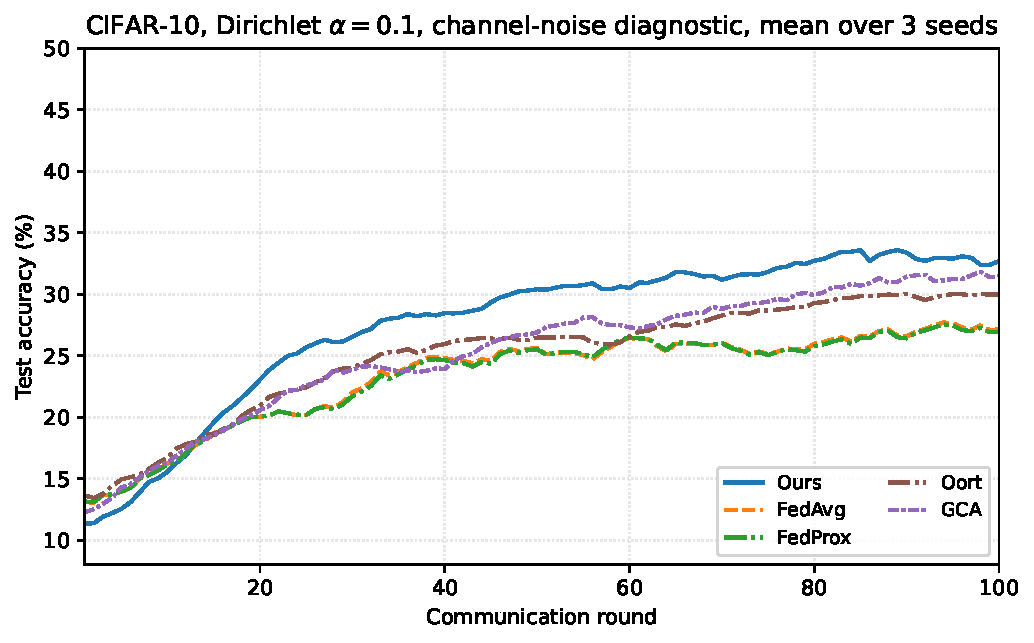
\includegraphics[width=\columnwidth]{figures/baseline_convergence.pdf}
    \caption{CIFAR-10 test accuracy ($\alpha=0.1$, $K=5$, $T=100$, channel-noise perturbation enabled). Curves show EMA-smoothed means over three seeds.}
    \label{fig:baseline_convergence}
\end{figure}

\subsection{Ablation Study}

Table~\ref{tab:ablation} separates the main design choices under the same nominal CIFAR-10 operating point.

\begin{table}[!htbp]
\centering
\caption{Ablation study.}
\label{tab:ablation}
\small
\setlength{\tabcolsep}{4pt}
\begin{tabular}{l|c}
\hline
\textbf{Variant} & \textbf{Last-5 acc.\ (\%)} \\
\hline
Full (SV + Queue + Energy) & 35.10 $\pm$ 0.81 \\
w/o SV                    & 31.03 $\pm$ 1.07 \\
w/o Queue                 & 33.05 $\pm$ 0.85 \\
w/o Energy (SV-only)      & \textbf{35.16 $\pm$ 3.91} \\
\hline
\end{tabular}
\end{table}

Removing the Shapley signal reduces the last-5 accuracy by 4.07 percentage points, while removing the virtual queue reduces it by 2.05 percentage points. This result shows that the Shapley contribution signal is the main factor for improving model accuracy in this ablation. The SV-only variant obtains a slightly higher mean accuracy than the full scheduler, but it does not include residual-energy feasibility and long-term queue accounting. Therefore, the full scheduler is the deployable energy-aware version.

In the tested setting, the energy-aware variants keep clients above the depletion threshold. The virtual queue provides an explicit long-term accounting mechanism. It penalizes persistent over-budget participation while preserving learning utility as much as possible.

\subsection{Heterogeneity Sensitivity}

Table~\ref{tab:sens_alpha} reports a three-seed sweep of the Dirichlet concentration parameter $\alpha \in \{0.1, 0.25, 0.5, 1.0\}$ at the same operating point ($T=100$, $V=10$). This sweep evaluates whether the scheduler is still useful when the data partition changes from highly skewed to more balanced.

\begin{table}[!htbp]
\centering
\caption{Heterogeneity sensitivity.}
\label{tab:sens_alpha}
\scriptsize
\setlength{\tabcolsep}{2.0pt}
\renewcommand{\arraystretch}{1.12}
\begin{tabular}{l|c|c|c|c}
\hline
\textbf{Method} & $\alpha=0.10$ & $\alpha=0.25$ & $\alpha=0.50$ & $\alpha=1.00$ \\
\hline
Ours & \textbf{32.35 $\pm$ 1.47} & \textbf{41.19 $\pm$ 0.59} & \textbf{46.24 $\pm$ 1.87} & \textbf{47.90 $\pm$ 0.51} \\
FedAvg & 26.34 $\pm$ 0.59 & 35.68 $\pm$ 2.68 & 42.03 $\pm$ 1.03 & 44.93 $\pm$ 0.52 \\
FedProx & 26.07 $\pm$ 0.91 & 35.61 $\pm$ 2.72 & 41.96 $\pm$ 0.94 & 44.99 $\pm$ 0.46 \\
Oort & 29.91 $\pm$ 2.39 & 39.98 $\pm$ 1.11 & 44.04 $\pm$ 1.22 & 43.27 $\pm$ 0.99 \\
GCA & 31.87 $\pm$ 1.19 & 40.40 $\pm$ 2.45 & 44.37 $\pm$ 0.14 & 43.43 $\pm$ 1.36 \\
\hline
\end{tabular}
\end{table}

The proposed scheduler achieves the highest mean last-5 accuracy for all tested heterogeneity levels. GCA is the strongest energy-aware comparator in this sweep. Ours improves over GCA by 0.48, 0.79, 1.87, and 4.47 percentage points at $\alpha=0.1$, $0.25$, $0.5$, and $1.0$, respectively. This indicates that the Shapley-guided queue scheduler remains competitive under both strongly skewed and more balanced partitions.

\subsection{Shapley Sampling-Budget Sensitivity}

Table~\ref{tab:budget} reports a single-seed diagnostic sweep over sampling budgets $M\in\{5,10,20,50\}$ for the CC-Neyman estimator. Increasing $M$ increases the number of validation-utility evaluations per round, but the accuracy trend is non-monotonic. This behavior can happen in an online scheduler, because a lower-variance contribution estimate does not automatically produce a better finite-round client-selection trajectory under non-IID data, channel variation, and queue penalties.

\begin{table}[!htbp]
\centering
\caption{Sampling-budget sensitivity.}
\label{tab:budget}
\scriptsize
\setlength{\tabcolsep}{2.2pt}
\begin{tabular}{c|c|c|c}
\hline
\textbf{Budget} & \textbf{Last-5 acc.\ (\%)} & \textbf{Final acc.\ (\%)} & \textbf{Eval./round} \\
\hline
$M=5$  & 31.99 & 33.89 & 10 \\
$M=10$ & \textbf{40.72} & \textbf{38.96} & 20 \\
$M=20$ & 33.63 & 34.39 & 40 \\
$M=50$ & 29.84 & 32.62 & 100 \\
\hline
\end{tabular}
\end{table}

The budget sweep supports using a moderate contribution-estimation budget. Moving from $M=5$ to $M=10$ improves last-5 accuracy in this diagnostic run. Larger budgets increase validation-utility evaluations but do not improve accuracy at this operating point. This single-seed sweep illustrates the evaluation-cost--accuracy tradeoff when selecting the Shapley sampling budget. Overall, the experiments show gains over baselines in the tested CIFAR-10 settings and illustrate how the energy queue and Shapley-sampling budget affect the scheduler.

\subsection{Channel-Noise Diagnostic}

The channel-noise component makes the simulations closer to wireless FL settings, where the received aggregate may be affected by natural propagation noise. Related wireless privacy studies show that channel noise can be incorporated into privacy-aware aggregation models when the physical-layer transmission and privacy budget are jointly considered \cite{yan2023otafedavgprivacy}. In this paper, the same equivalent clipped noisy-release condition is applied to all compared schedulers. Therefore, the reported gains mainly come from client scheduling rather than different perturbation levels.

\section{Conclusion}
\label{sec:conclusion}

This paper studied client scheduling for synchronous cross-device FL under non-IID data, wireless channel variation, and long-term energy constraints. We proposed a Shapley-guided channel- and energy-aware scheduler. The scheduler maintains persistent contribution estimates through a complementary-contribution sampler, evaluates residual battery and channel states at each round, and uses virtual energy queues to penalize repeated energy overuse. The resulting score helps the server prefer informative clients when they are feasible and timely, while keeping an explicit accounting mechanism for long-horizon energy pressure.

We also incorporated a lightweight channel-noise diagnostic motivated by the natural noise introduced during wireless propagation. Uploaded updates are clipped to bound the aggregate perturbation scale. Receiver-side channel uncertainty is modeled as equivalent Gaussian perturbation on the released aggregate. This design provides a common noisy wireless-release condition for evaluating the proposed scheduler and the baselines under the same perturbation scale.

Experiments on CIFAR-10 show that the proposed scheduler improves over random-selection and utility-based baselines in a difficult non-IID regime. Ablation studies indicate that the Shapley signal improves accuracy, while the virtual queue provides the energy-accounting mechanism required by the deployable scheduler. Diagnostic sensitivity experiments further show how performance changes with data heterogeneity and contribution-estimation budget. Overall, the results support the scheduler as a candidate mechanism for balancing contribution, channel opportunity, and energy sustainability in resource-constrained FL.

Future work will extend the framework to asynchronous FL, richer device heterogeneity, tighter theoretical links between online complementary-contribution estimation and score-based stochastic scheduling, and protocol-level integration of secure aggregation with contribution evaluation.

\bibliographystyle{IEEEtran}
\bibliography{references}

\end{document}
